\documentclass[a4paper, notitlepage]{article}

\usepackage{hyperref}
\usepackage[T1]{fontenc}
\usepackage{lmodern}
\usepackage{listings}
\usepackage{capt-of}
\usepackage{graphicx}





\newcommand{\flame}{\texttt{flame}}
\newcommand{\fuel}{\texttt{fuel}}

\begin{document}

\title{\flame\ user manual}
\author{Sirio Belli}
\maketitle



% ***********************************************************************************************


\section{Introduction}

\flame\ is an IDL data reduction pipeline for near-infrared multi-object spectroscopy. Although written specifically for the LUCI instrument at LBT, it has been designed in a modular way and can be easily adapted to work with the data produced by different instruments.



% ***********************************************************************************************


\section{Installation}

\subsection{Requirements}

The following three external IDL libraries must be installed before running \flame.
\begin{enumerate}
\item NASA's \href{http://idlastro.gsfc.nasa.gov/}{IDL Astronomy User's Library};
\item David Fanning's \href{http://www.idlcoyote.com/code_tips/installcoyote.php}{Coyote Library};
\item Craig Markwardt's \href{https://www.physics.wisc.edu/~craigm/idl/fitting.html}{mpfit} (only the mpfit.pro and mpfit2dfun.pro files are needed for \flame). 
\end{enumerate}
Make sure to have the most recent versions of these libraries (at least more recent than the January 2016 release).

Other third-party routines used by \flame\ are included in the distribution, in the flame/lib/ directory. These are the bspline routines from the \texttt{idlutils} library.


\subsection{Download}

Download the \flame\ IDL code from \url{https://github.com/siriobelli/flame}. Either save it in the directory where you keep your IDL code, or add the flame/ directory to the IDL path. No other step is necessary.


% ***********************************************************************************************


\section{Setting up the Data Reduction}

Go to the directory that you want to use for the reduction of a data set (it is recommended to create a new directory for this purpose). Then:
\begin{itemize}
\item Copy the file \texttt{flame\_driver.pro} from the \flame\ directory to the current directory.
\item Create a directory where the intermediate files produced by the pipeline will be saved (e.g., intermediate/)
\item Create a directory where the final output of the data reduction will be saved (e.g., output/)
\item \emph{(optional)} Create a directory that will contain the input files (e.g., input/)
\item Create an ASCII file with, in each line, the full name (including absolute path) of a raw science file (e.g., input/science.txt)
\item \emph{(optional)} Create an ASCII file with the names of the flat field frames (e.g., input/flats.txt)
\item \emph{(optional)} Create an ASCII file with the names of the dark frames (e.g., input/darks.txt)
\end{itemize}


\subsection{Standard options}

The data reduction is entirely controlled via the driver file \texttt{flame\_driver.pro}. Open the local copy with a text editor and have a look at the code.

The driver file is divided into parts. The first part is the preamble, and set the input parameters for this particular data set. The second part is the data reduction, and does not require any input from the user.

The data reduction in \flame\ consists of a series of steps, which are represented by individual routines in the driver. The information is carried from one routine to the next via the use of only one structure, named \fuel, which contains all the input parameters set by the user in the preamble.

First we need to create fuel!

First, we need to define the directories for intermediate and final outputs:
\begin{lstlisting}
fuel.intermediate_dir = 'intermediate/'
fuel.output_dir = 'output/'
\end{lstlisting}
Note that these definitions use relative paths, and will work only if you run the driver from the directory immediately above intermediate/ and output/. It is safer to always use absolute paths (e.g., /scr/observing/run\_1/mask\_1/output/).

Now we define the input files:
\begin{lstlisting}
fuel.science_filelist = 'input/science.txt'
fuel.darks_filelist = 'input/darks.txt'
fuel.flats_filelist = 'none'
\end{lstlisting}
In this example the flat field frames are not available and the corresponding field is set to \textquoteleft none\textquoteright. The same can be done for the dark frames. The science frames must, of course, always be specified.

Reference star etc.
\begin{lstlisting}
fuel.startrace_y_pos = [547, 560]
\end{lstlisting}

In alternative, need to specify the dithering pattern:
\begin{lstlisting}
fuel.startrace_y_pos = [0, 0]
fuel.dither_filelist = 'input/dither.txt'
\end{lstlisting}



\subsection{Advanced options}

\subsubsection{Reduce only one slit}

Because reducing one entire slitmask can take a long time, especially for deep observations with a large number of frames, \flame\ offers the possibility to reduce only one slit. This is particularly useful when observing, so that quick decisions can be made based on the final reduction of a representative object. To reduce only one slit we need to specify the slit index (starting from 1). For example if we are interested in the third slit:
\begin{lstlisting}
fuel.reduce_only_oneslit = 3
\end{lstlisting}
The default value for fuel.reduce\_only\_oneslit is zero, which means that all the slits will be reduced.

\subsubsection{Specify the x coordinates for the reference star}

\subsubsection{Longslit observations}



\subsection{Initialization}

\begin{lstlisting}
flame_initialize_luci, fuel=fuel
\end{lstlisting}





% ***********************************************************************************************



\section{Running the Data Reduction}

Once the first part of the driver file has been edited, the data reduction is fully automatic. One way to run \flame\ at this point would be to execute the driver directly from the command line:
\begin{lstlisting}
idl flame_driver.pro
\end{lstlisting}
Another possibility, which allows some interaction and testing, is to copy line-by-line the content of the driver file onto an interactive IDL session. This way one can explore the output files and the fuel structure after every step.

The second part of the driver file contains eight steps or modules, which we are going to examine in detail in this section. Every module is an IDL routine whose name starts with \texttt{flame\_} and which is saved in a .pro file with the same name in the directory flame/pro/. All modules accept (and require) only one argument, which is the \fuel\ structure, so that the IDL code for each module looks the same:
\begin{lstlisting}
flame_modulename, fuel=fuel
\end{lstlisting}

Every module edits the fuel structure and/or outputs files in the intermediate directory. Only the last module, which creates the final results, saves the output files in the output directory.



% ---------------------------------------------------
\subsection{\texttt{flame\_diagnostics}}

The first step produces important diagnostics which will be used by the successive modules. These diagnostics can also be helpful to the user to assess the quality of the observations, and can be run in real time while observing, ideally after every new frame or frame pair has been taken.

\begin{figure}[htbp]
\centering
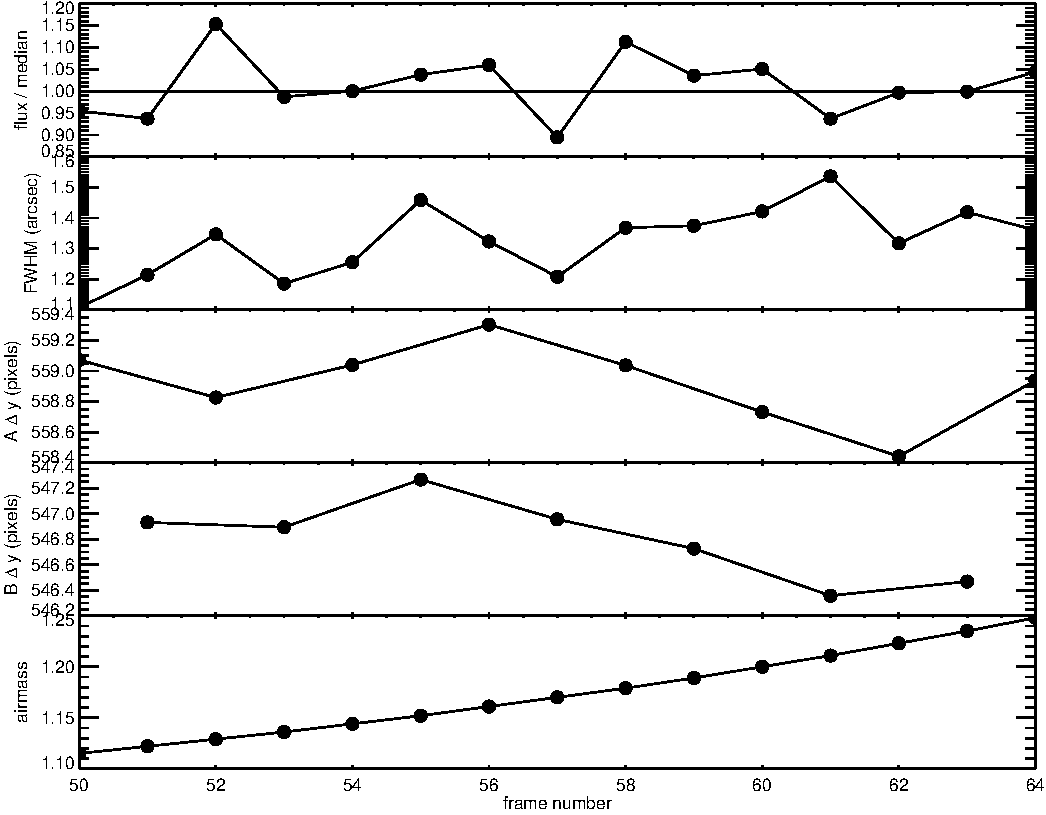
\includegraphics[width=0.9\textwidth]{diagnostics}
\caption{Example of diagnostics plot.}
\label{fig:diagnostics}
\end{figure}

Starting with the y coordinates specified by the user in fuel.startrace\_y\_pos, this module detects the reference star position on each frame, and identifies which frames belong to the $A$ and which to the $B$ position (and assign an $X$ position when no star trace is found). Then, for each frame a Gaussian profile is fit to the star trace, from which the flux, vertical position and FWHM are measured. In addition, the airmass value is measured from the FITS header of each frame.

All these quantities are saved in the substructure fuel.diagnostics. They are also output in the ASCII file diagnostics.txt, and plotted as a function of the frame number in the file diagnostics.ps. One example of such file is shown in Figure \ref{fig:diagnostics}. Becasue of the dithering, the vertical position is shown in different panels for the $A$ and the $B$ frames.

The diagnostics plots can be used to judge the trend of transmission (including the effect of cloud cover), seeing, and drift. In addition to help the user make informed decisions while observing, these measurements are also useful to identify the bad frames that should be excluded from the final data reduction.



% ---------------------------------------------------
\subsection{\texttt{flame\_quickstack}}

The second step produces a FITS file (quickstack\_A-B.fits) which is the difference of a stack of the $A$ frames and a stack of the $B$ frames (as defined in the previous module). This step is also useful while observing, since the simple $A-B$ subtraction often yields a decent sky removal which allows the detection of faint continuum traces or emission lines.

The sole goal of this module is to allow a quick look at the data. This step can be skipped with no consequences for the remaining parts of the data reduction.



% ---------------------------------------------------
\subsection{\texttt{flame\_correct}}

This module apply a number of correction to the raw science frames. First, the bad pixel mask is generated from the input dark frames. If no dark frames were supplied, then the default bad pixel mask, stored in flame/data/, is used.

The following corrections are applied:
\begin{itemize}
\item Linearity correction: the value of each pixel is corrected to take into account the non-linear response of the detector. The correction is a polynomial function with instrument-specific coefficients, which are determined during the initialization.
\item Bad pixels are set to NaN.
\item The flux ofeach pixel is multiplied by the gain. This converts the flux units from ADUs to electrons.
\end{itemize}

Each of the corrected science frame is then saved in the intermediate directory.


% ---------------------------------------------------
\subsection{\texttt{flame\_getslits}}




% ---------------------------------------------------
\subsection{\texttt{flame\_wavecal}}



% ---------------------------------------------------
\subsection{\texttt{flame\_skysub}}


% ---------------------------------------------------
\subsection{\texttt{flame\_rectify}}



% ---------------------------------------------------
\subsection{\texttt{flame\_combine}}




% ***********************************************************************************************






\end{document}